% main.tex
%
% (c) 2024 Lukas Schöpf, OST Ostschweizer Fachhochschule
%


\documentclass[hidelinks]{report}
% öffnet packages.tex
%
% packages.tex -- TeXfiles
%
% (c) 2023 Jakob Gierer & Lukas Schöpf, OST Ostschweizer Fachhochschule
%


%packages
\usepackage[english]{babel}
\usepackage[utf8]{inputenc}
\usepackage{csquotes}
\usepackage[T1]{fontenc}
\usepackage[backend=biber, style=ieee]{biblatex}
\usepackage{hyperref}
\usepackage{amsmath,amscd}
\usepackage{amssymb}
\usepackage{amsfonts}
\usepackage{amsthm}
\usepackage{amsmath}
\usepackage{makecell}
\usepackage{txfonts}
\usepackage{graphicx}
\usepackage{tabularx}
%\usepackage{subcaption}
\usepackage{subfig}
\usepackage[many]{tcolorbox}
\usepackage[acronym]{glossaries}
\usepackage{fancyhdr}
\usepackage[toc,page]{appendix}
\usepackage[headheight=12.1pt]{geometry}
\usepackage[english]{cleveref}
\usepackage{lmodern}
\usepackage{booktabs}
\pagestyle{fancy}


%Für Test
%\usepackage{blindtext}


\addbibresource{references.bib}
\bibliography{references}
\makeglossaries
%
% acro.tex
%
% (c) 2024 Lukas Schöpf, OST Ostschweizer Fachhochschule
%
\newacronym{ost}{OST}{Ostschweizer Fachhochschule}
\newacronym{snr}{SNR}{Signal to Noise Ration}
\newacronym{cnn}{CNN}{Convolutional Neural Networks}
\newacronym{clip}{CLIP}{Contrastive Language-Image Pre-training}
\newacronym{align}{ALIGN}{A Large-scale ImagGe and Noisy-text embedding}
\newacronym{sam}{SAM}{Segment Anything}
\newacronym{hef}{HEF}{Hailo Executable File}
\newacronym{dfc}{DFC}{Dataflow Compiler}
\newacronym{pca}{PCA}{Principal Component Analysis}
\newacronym{har}{HAR}{Hailo Archive}
\newacronym{tse}{TSE}{Tiled Squeeze-and-Excite}
\newacronym{rnn}{RNN}{Recurrent neural network}
\newacronym{api}{API}{application programming interface}
\newacronym{gpu}{GPU}{Graphics processing unit}



% name des tex-file Reinschteiben welches man bearbeitet
%\includeonly{text/Entwicklung} % Auskommentiern um ganzes Dokument zu setzen

\begin{document}
    \pagenumbering{Roman}
     % öffnet titlepage.tex
    %
% titlepage.tex -- TeXfiles
%
% (c) 2024 Jakob Gierer & Lukas Schöpf, OST Ostschweizer Fachhochschule
%


\begin{titlepage}
    % Bigger symmetric margins
    \newgeometry{
        outer = 3cm, inner = 3cm, top=5cm,bottom=6cm
    }
    \centering
%    \vspace{4cm}

    % Titel
    {\huge \bfseries \sffamily Scene Understanding \par
     \normalfont\itshape On-Site Scene Understanding with Edge AI \par}
    \vspace{1cm}

    % Autoren
    {\large \textsl{Lukas Schöpf}}
    \par
    \vspace{1cm}

    % Informationen über Hochschule
    {\textsc Master Project \par}
    {Ostschweizer Fachhochschule \par}
    \today
    \vfill
    
    % Titelbild
    % Beispiel
%    \begin{figure}[h]
%        \centering
%        \includegraphics[width=3cm]{example-image-c}
%    \end{figure}

    % Oder Tikz
    % \resizebox{.9\linewidth}{!}{
        %   \input{figures/tikz/}
        % }
    \vfill

    % % Wichtige Informationen
    % \begin{tabular}{rl}
    %     \bfseries\sffamily Thema & Audioklassifizierung \\
    %     \bfseries\sffamily Fachgebiet          & Digitale Signalverarbeitung \\
    %     \bfseries\sffamily Betreuer       & Hannes Badertscher, Patrik Müller \\
        
    % \end{tabular}
    \restoregeometry    
\end{titlepage}


    %%
% Abstrakt.tex
%
% (c) 2023 Jakob Gierer & Lukas Schöpf, OST Ostschweizer Fachhochschule
%

\chapter*{Abstrakt}
Test
	
	
    %%
% Dankessagung.tex
%
% (c) 2023 Jakob Gierer & Lukas Schöpf, OST Ostschweizer Fachhochschule
%

\chapter*{Danksagung}

Wir möchten diese Gelegenheit nutzen, um unseren aufrichtigen Dank all jenen auszudrücken, die uns während der Erstellung unserer Bachelorarbeit unterstützt und inspiriert haben.
\vspace{11pt}

\noindent
Ein besonderer Dank gilt auch unseren Betreuungspersonen, Patrik Müller und Hannes Badertscher.
Ihre fachliche Expertise, ihre Geduld und ihre Ratschläge waren von unschätzbarem Wert für den Erfolg unserer Arbeit.
Wir sind dankbar für die konstruktive Kritik und die Unterstützung, die sie uns entgegengebracht haben.
\vspace{11pt}

\noindent 
Ein herzliches Dankeschön geht auch an Florian Baumgartner und Alain Keller, die uns bei der Anpassung und Benutzung ihres Codes unterstützten. 
\vspace{11pt}

\noindent
Ausserdem möchten wir unseren Familien für das Korrekturlesen unserer Bachelorarbeit danken. 
    \pagestyle{plain}
    \tableofcontents
    {
    	\linespread{0.7}\selectfont{}
    	\glsnogroupskiptrue
    	\printglossary[type=\acronymtype]
    }
    % \printglossary[type=\acronymtype]
    % add common macros
    %
% macros.tex
%
% (c) 2023 Jakob Gierer & Lukas Schöpf, OST Ostschweizer Fachhochschule
%

% Kopfzeilen
%
\renewcommand{\headrulewidth}{0.4pt}
\renewcommand{\chaptermark}[1]{%
    \markboth{#1}{}
}
\renewcommand{\sectionmark}[1]{
    \markright{#1}
}

\rhead{\leftmark}
\lhead{\rightmark}

%to set Numbers in Circles use \kreis{}
\newcommand{\kreis}[1]{\unitlength1ex
    \begin{picture}(2.5,2.5)
        \put(0.75,0.75){\circle{2.5}}\put(0.75,0.75){\makebox(0,0){#1}}
\end{picture}}

%for different colored Text
\definecolor{YellowOrange}{RGB}{255, 159, 43}
\definecolor{RoyalBlue}{RGB}{0, 122, 255}
\definecolor{ForestGreen}{RGB}{18, 159, 87}

% Beispiel umgebung erstellen
\newcounter{satz}[chapter]
\newenvironment{beispiel}{%
    \refstepcounter{satz}
    \begin{proof}[Beispiel \arabic{chapter}.\arabic{satz}]%
        \renewcommand{\qedsymbol}{$\bigcirc$}
    }{\end{proof}}
    \newpage
    \pagenumbering{arabic}
    \pagestyle{fancy}
    % ==================================================
    % Beispiel um externe Textdokumente hinzuzufügen 
    % \input{file}
    \chapter{Introduction}
Hexagon AB\cite{hexagon} is a global player in digitisation technology and specializes in measurement and positioning systems.
Hexagon’s laser scanning devices produce point cloud data of the environment and capture images through additional cameras integrated into their scanners.
A challenge in Hexagon’s laser scanning applications is to build ever smarter scanning devices which have better understanding of the scenes they are placed in by preferably pre-processing the environment
information they record directly in the field.

The goal of this project is to work towards integration of enhanced scene understanding capabilities into the scanning application’s edge devices.
A scanner should, for example, be able to classify a scene on various hierarchical levels and with increasing level of detail, namely indoor vs. outdoor, construction site 
vs. completed building (eventually inferring even the degree of building completion), office complex vs.
family house, small vs. big room, kitchen vs. bathroom, bathroom with vs. without bathtub, etc.

To this end, this project aims at evaluation, implementation, and test of smaller machine learning models
suitable for an Edge AI platform to demonstrate that corresponding classification tasks
could be embedded on board of a laser scanner in the future.
    \chapter{Task definition}
This work shall include the following work packages:
\subsection*{State-of-the-art in Scene understanding}
\begin{itemize}
    \item Get familiar with the state-of-the-art concerning machine learning/deep learning models for environment recognition and scene understanding by reading the relevant scientific papers, covering foundation models like SAM\cite{sam} or CLIP \cite{clip}.
    \item Understand the working principles of existing approaches, especially CLIP and TinyCLIP\cite{tinyclip}, in detail.
    \item Gather experience with CLIP-based models by experimenting on suitable available datasets and code (openly available or provided by Hexagon) within a PC-environment (e.g., Python-based application). The dataset provided by Hexagon provides over 1000 panoramic images from at least five different classes.
\end{itemize}

\subsection*{Hardware accelerator Overview}
\begin{itemize}
    \item Perform a brief market analysis to collect an updated view of currently active players (universities, startups, and larger companies) for the provision of AI hardware accelerators with M.2 interface capabilities (like the one of Raspberry Pi AI Kit), which could be effectively used for a CLIP-based approach like in our project.
    \item Set up the Raspberry Pi AI Kit and its toolchain, and specifically compare the Hailo AI accelerator with the other hardware accelerators found from above.
\end{itemize}

\subsection*{CLIP model on Edge AI Platform}
\begin{itemize}
    \item Integrate a state-of-the-art machine learning algorithm like TinyCLIP on Raspberry Pi AI Kit (typically using Python on Raspberry Pi and C/C++ for Hailo AI accelerator).
    \item Test the performance of the implementation (using meaningful metrics) and run benchmarking to evaluate differences (e.g., in performance) when computing CLIP in the cloud vs. on the edge.
    \item Create a proof-of-concept with the Raspberry Pi AI Kit platform that demonstrates feasibility of the use case by processing realistic datasets from Hexagon.
\end{itemize}

\subsection*{Enhanced Proof-of-Concept}
\begin{itemize}
    \item Add some own improvements regarding performance, reliability, or generalization to the existing AI models and/or platform ports, considering quantization, pruning, architecture modifications, dataset processing, training, and optimized hardware deployments (allocation).
    \item Generalize the implementation to arrive at a unified Edge AI platform framework that can operate with ideally any other AI hardware accelerator card providing a M.2 slot interface.
    \item \textit{Optionally} Expand the used machine learning pipeline to support multi-label classification.
    \item \textit{Optionally}  Extend the given framework and platform to test other foundation models (like SAM) in an edge deployment.
    \item \textit{Optionally}  Explore the possibility to incorporate user feedback and a respective feedback mechanism on the platform, which may offer valuable continuous updates in an effort towards online learning.
\end{itemize}
    \chapter{Literature Review}

This literature review explores relevant papers in the field of scene understanding and those how work like CLIP.  
Current state-of-the-art techniques rely on deep learning models for scene understanding tasks.  
The primary objective of scene understanding is to extract semantic information from a given scene.  
This serves as the foundation for various applications such as surveillance, autonomous driving, road safety, vision-guided mobile navigation, and more.  
The significance of this field has grown alongside the rapid advancements in neural networks in recent years.  

A significant portion of the literature focuses on applications in autonomous driving \cite{sceneunderstandingautdriving1}.  
In early research, \acrfull{cnn} models, such as SegNet \cite{SegNet}, were predominantly used for scene understanding tasks.  
However, with the introduction of transformers \cite{attentionisallyouneed}, many researchers transitioned to this newer architecture.  
Subsequently, cross-modal networks such as CLIP \cite{clip} and ALIGN \cite{ALIGN} emerged.  
These networks utilize a text and image encoder to learn and predict relationships between image-text pairs.  
Their pre-training enables users to fine-tune them for specific tasks without the need to train an entirely new network.  
For instance, fine-tuning can be achieved by adding a linear layer or employing more sophisticated methods like feature distillation \cite{finetuneclip}.  
Other strategies, such as linear probing \cite{linearprobeclip} and the CLIP adapter \cite{clipadapter}, have demonstrated improvements in task-specific performance.  

Segmentation of scenes can also enhance the ability to observe and analyze specific objects within an image.  
Foundational models like \acrfull{sam} \cite{sam} can be employed for image pre-processing or feature extraction, aiding in these tasks.  

To address the challenges of deploying large networks in resource-constrained environments, techniques such as knowledge distillation have been developed.  
These methods significantly reduce network size while maintaining functionality.  
For example, TinyCLIP \cite{tinyclip} reduces the original network size by 75\%, enabling its use on limited platforms and facilitating edge computing.  

    %
% clip.tex
%
% (c) 2024 Lukas Schöpf, OST Ostschweizer Fachhochschule
%

% DeepL corrected
% explain Resnet and transformer

\chapter{Cross-modal networks
    \label{chapter:crossmodalnetworks}}
    Multimodal deep learning is the study of models that learn from multiple modalities.
    For example, a human can use both vision and hearing to identify an object or a person.
    Cross-modal deep learning uses data from one modality to improve performance in another.
    For example, if a person looks at a picture of a bird and listens to the bird's song, they might be able to identify the bird.
    
    Its most impressive feature is the ability to perform well on data on which the model has not been trained.
    This ability is called zero-shot capability, which is derived from N-shot capability.
    N-shot capability describes how many training samples of a particular class a model needs to classify it correctly.

    In this work, cross-modal networks are used to find relationships between images and text.
    Networks trained for this task are called contrastive language-image pre-training models.
    Most cross-modal networks built for this task consist of a text encoder and an image encoder.

    \section{Base networks}
    To understand corss-modal netwroks we first have to understand thier components.
    Most of them use a transformers as encoders but some can use ResNets.
    Information for this section are taken from the corresponding paper and \cite{clipexplain}.
    
    \subsection{ResNet
    \label{crossmodalnetworks:sec:resnet}}
    ResNet's were introduced in \cite{resnetpaper}.
    A ResNet uses residual blocks (\cref{fig:crossmodalnetworks:resblock}).
    These blocks have residual conections between some layers.
    This allows information to bypass whole layers if the layers are not needed.
    These conections stabilizes training and convergence of deep neural networks.
    ResNets original motivation was to have better image processing capabilities then \acrfull{cnn}.
    Big and deep transformer models like GPT models from Open AI also use these conections to get better results.

    \begin{figure}[h]
        \centering
        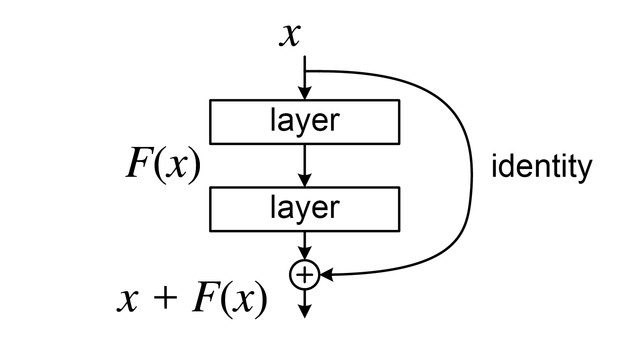
\includegraphics[width=0.55\textwidth]{Images/crossmodalnetworks/ResBlock.png}
        \caption{Image of a ResNet block.\cite{resnetpaper}}
        \label{fig:crossmodalnetworks:resblock}
    \end{figure}

    \subsection{Transformer}

    The transformer is first meantioned in \cite{attentionisallyouneed}.
    Before transformers \acrfull{rnn} were used to process sequential data.
    A mechanism called attention was used to get information about the context of a sequenz.
    The transformer was a revolution because it uses a  block called self attention.
    With this block the need for a \acrshort{rnn} is obsolet.
    \acrshort{rnn} are hard to train because of a effect called vanishing or exploding gradient.
    They are also hard to parallelize.
    These effect's no longer occure when using a transformer.


    To use a transformer the input has first to be split in tokens.
    These tokens consist of text snippets or in the case of a vision transfomer patches of a picture(see \cref{fig:crossmodalnetworks:visiontransformer}).
    These tokens then get embedded into a high dimensional vector space.
    In case of CLIP Vit32 visual encoder the vector has 1024 dimensions.
    Additionally the vectors get a postitional embedding.
    Next a combination of self attention block and feed forward is used to process the tokens (see \cref{fig:crossmodalnetworks:transformer}).
    Mutliple of these block get concantenated.

    \begin{figure}[]
        \centering
        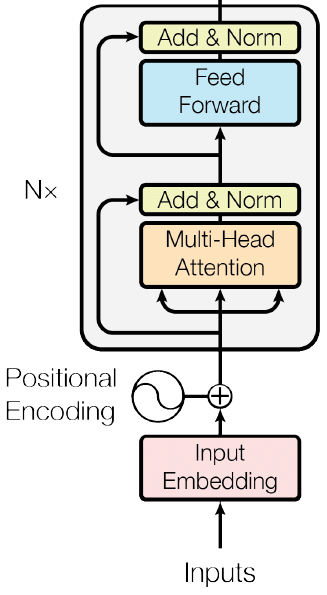
\includegraphics[width=0.25\textwidth]{Images/crossmodalnetworks/The-Transformer-encoder-structure.png}
        \caption{Image of a transformer which in the case of CLIP is used as a text encoder\cite{fig:encoder}}
        \label{fig:crossmodalnetworks:transformer}
    \end{figure}

    \begin{figure}[]
        \centering
        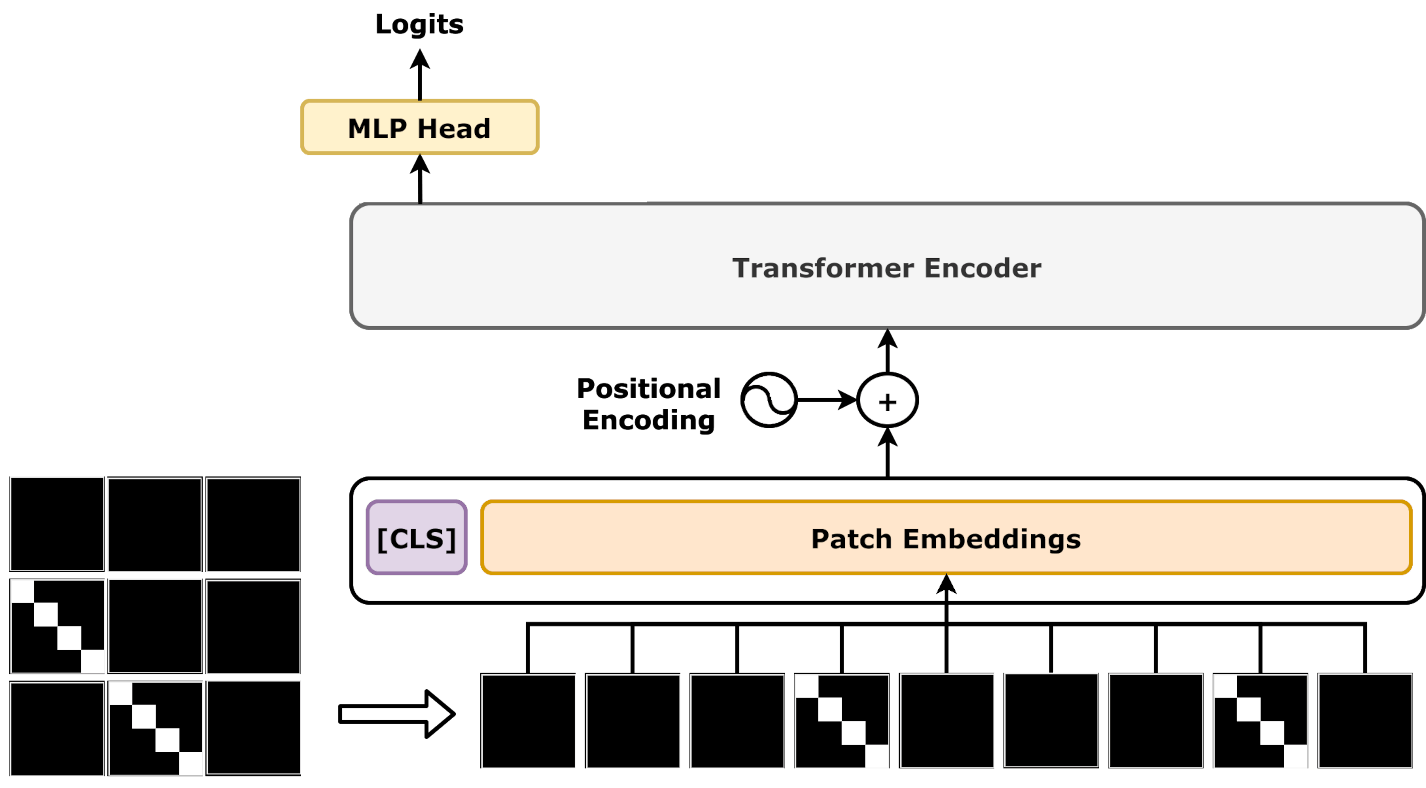
\includegraphics[width=0.6\textwidth]{Images/crossmodalnetworks/Vision_Transformer.png}
        \caption{Vision transforme architecture\cite{vitwikipedia}}
        \label{fig:crossmodalnetworks:visiontransformer}
    \end{figure}


    \section{Text encoder}
    The text encoder is in most cases a transformer.
    It encodes a given text into a high-dimensional vector space.
    This high dimensional vector space allows the encoder to correctly classify unseen classes because their vector is close to related classes.
    In theory, the closer two words are related, the closer their embedding vectors are to each other.
    An example of this can be seen in \cref{fig:crossmodalnetworks:3demb}, where \Acrfull{pca} is used to reduce the dimensions of the embedding vectors.
    Cat and dog are close together.

    \begin{figure}
        \centering
        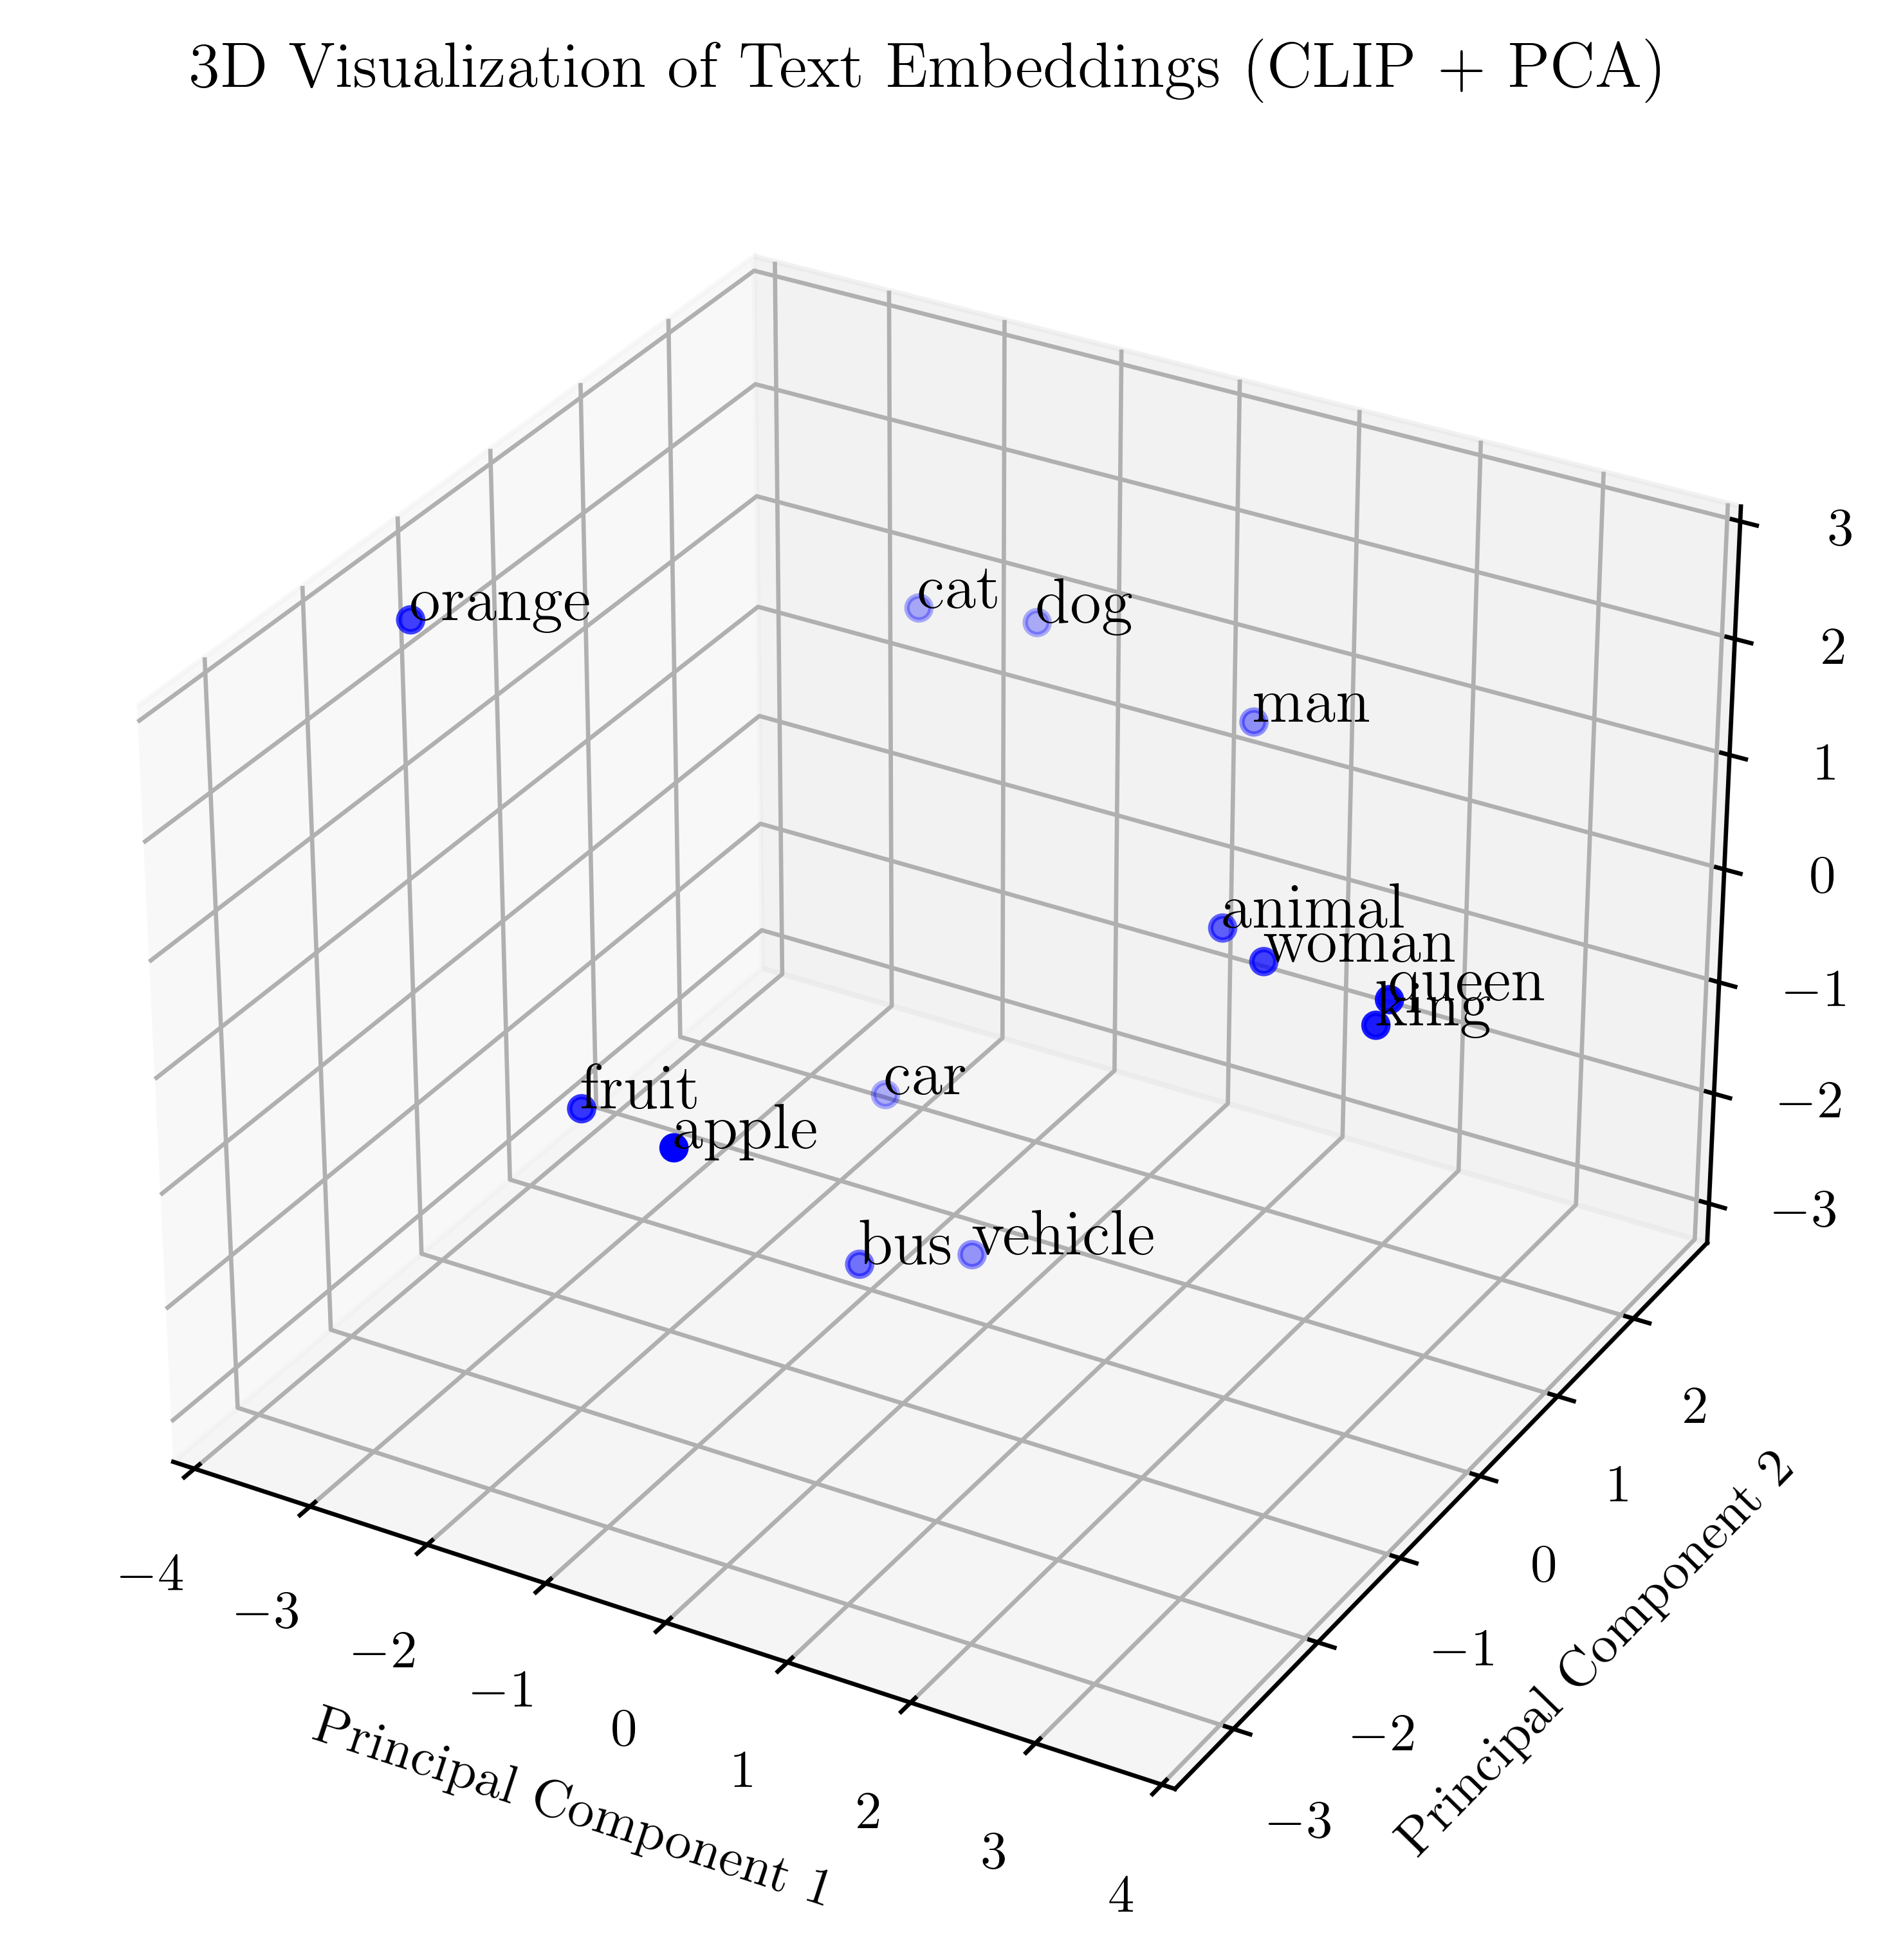
\includegraphics[width = 0.8\textwidth]{Images/crossmodalnetworks/3DEmbedding.png}
        \caption{Example of text embedding using CLIP and \Acrshort{pca}}
        \label{fig:crossmodalnetworks:3demb}
    \end{figure}
    
    \section{Image encoder}
    In most cases, the image encoder consists of a vision transformer\cite{Vis_N_Grams}.
    Like a text encoder, the vision encoder encodes an image in a high-dimensional vector space.
    A vision transformer needs an image in a specific dimension.
    For this reason, an image encoder is a pair of vision transformer and preprocessor that transforms an image into the right dimensions for the vision transformer.

    
    \section{Contrastive Language-Image models
        \label{section:languageimagemodels}}
        This section examines some models that use contrastive language-image pretraining.
        Most of the information in this section is taken from \cite{cliplikeweb} and the related papers.

        Contrastive techniques take paired inputs from two modalities (e.g. an image and its caption).
        Both inputs are embedded in their own embedding space.
        The aim is for such a pair to be represented by its corresponding encoder in a similar embedding.
        Language-image describes the two modalities used by the model.
        Most of these models are pre-trained.
        Pre-training means that the model has been trained on a large and universal dataset.
        For a specific application, a pre-trained model can be fine-tuned to better perform on its specific task.

        \subsection{CLIP
            \label{section:clip}}
        \acrfull{clip} \cite{clip} is a cross-modal model from openAI\cite{openai} that can tell how well a given image and text match.
        It can be used with a variety of image and text encoders.
        It is trained on a large dataset consisting of 400 million image-text pairs.
        It has been shown to outperform some of the best known models in classifing images.
        Many other models use CLIP as a base and build better models from it.

        \begin{figure}[]
            \centering
            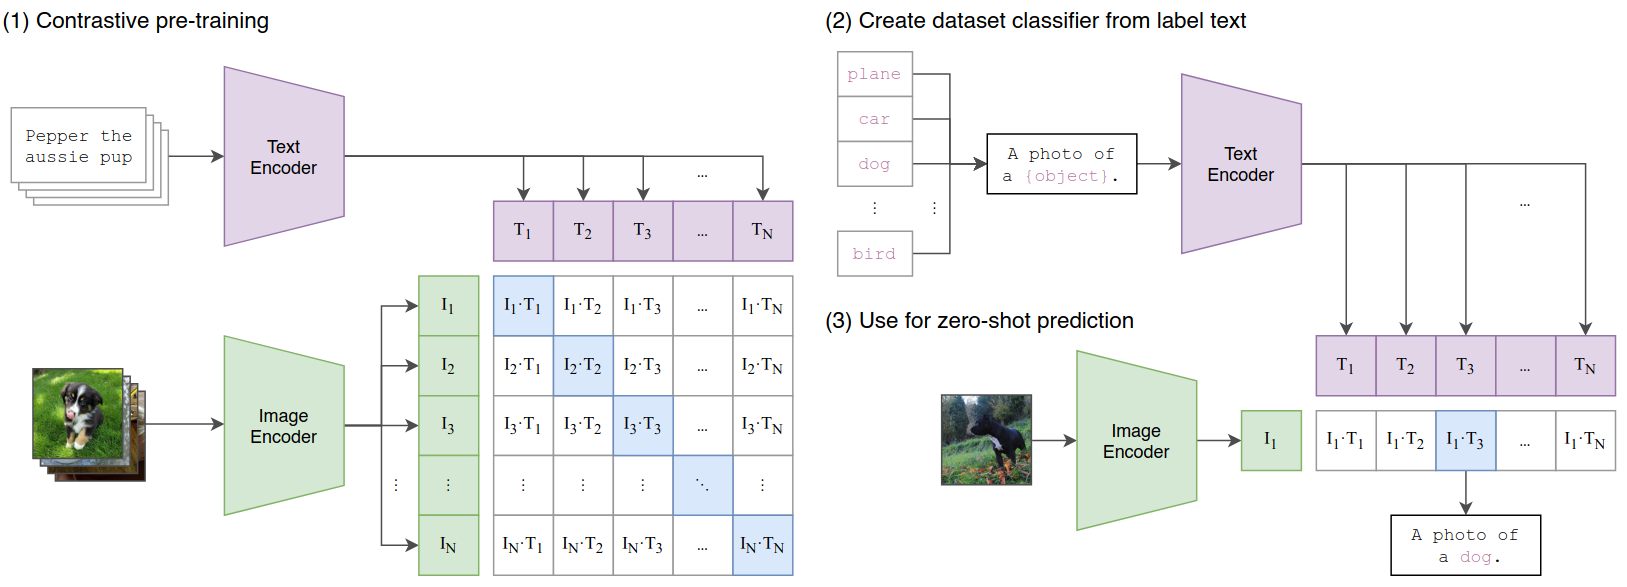
\includegraphics[width=\textwidth]{Images/crossmodalnetworks/OpenAICLIP.png}
            \caption{A picture from the \acrshort{clip} paper by OpenAI \cite{clip}.}
            \label{fig:crossmodalnetworks:openaiclip}
        \end{figure}

        \subsection{ALIGN
            \label{section:align}}
        \acrfull{align}\cite{ALIGN} was released shortly after \acrshort{clip}.
        Rather than relying on small and image caption datasets, \acrshort{align} uses a dataset of \(1.8\) billion pairs of image and alt-text pairs (e.g. in \cref{fig:crossmodalnetworks:alignepairs}).
        These alt-text descriptions are much noisier than captions.
        The authors apply basic filtering to remove duplicates, images with more than 1000 associated alt-texts, and uninformative alt-texts (either too frequent or containing rare tokens), but avoid expensive filtering operations.
        With just these simple steps, ALIGN meets or exceeds the state of the art for several zero-shot and fine-tuning tasks.
        \begin{figure}
            \centering
            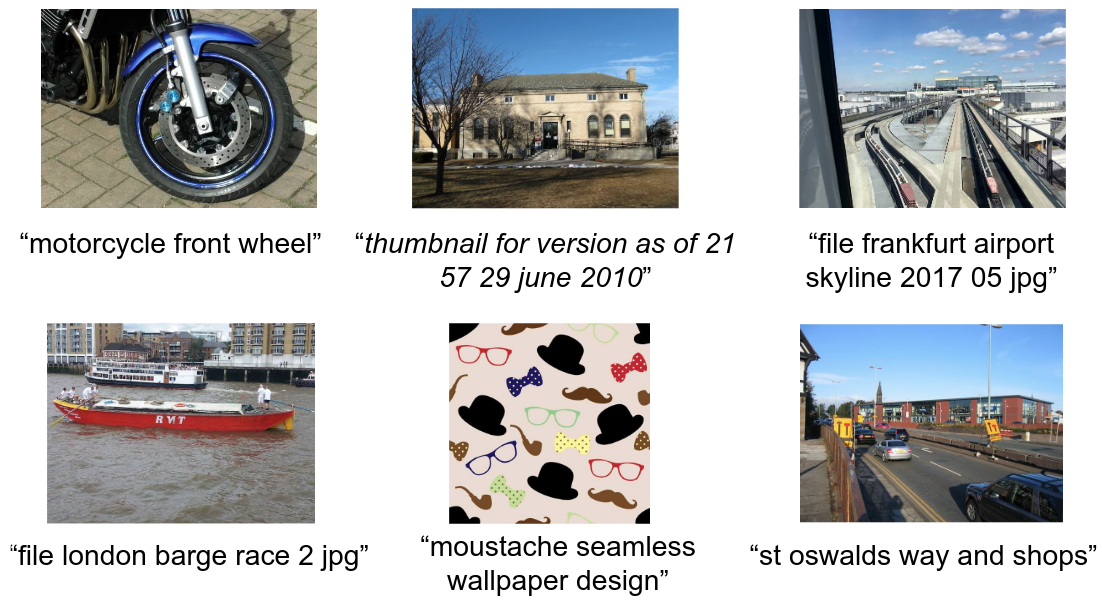
\includegraphics[width=\textwidth]{Images/crossmodalnetworks/examplepicsalign.png}
            \caption{Example of alt-text image pairs from the train dataset from \acrshort{align}\cite{ALIGN}}
            \label{fig:crossmodalnetworks:alignepairs}
        \end{figure}

        In a test for this paper, \acrshort{align} was much slower than CLIP to compute a zero-shoot evaluation on the CIFAR100\cite{cifar100} dataset.
        For 1 prediction, \acrshort{align} takes 70 times longer than \acrshort{clip} (see \cref{tab:clipaligntest}).
        Both networks are not fine-tuned. The highest predicted label is used. Due to the slow interference, ALIGN was stopped after processing 35\% of the dataset.

        \begin{table}
            \centering
            \begin{tabular}{lll}
                \hline
            \textbf{Measurment}&\textbf{ALIGN}&\textbf{CLIP}\\\hline
            Accuracy& 48.9\% & 61.7\%\\
            Speed(seconds per iterarion)&  2.16&  0.02\\ \hline
            \end{tabular}
            \caption{First test on CIFAR100.}
            \label{tab:clipaligntest}
        \end{table}

        \subsection{TinyCLIP
            \label{section:tinyclip}}
        \begin{figure}
            \centering
            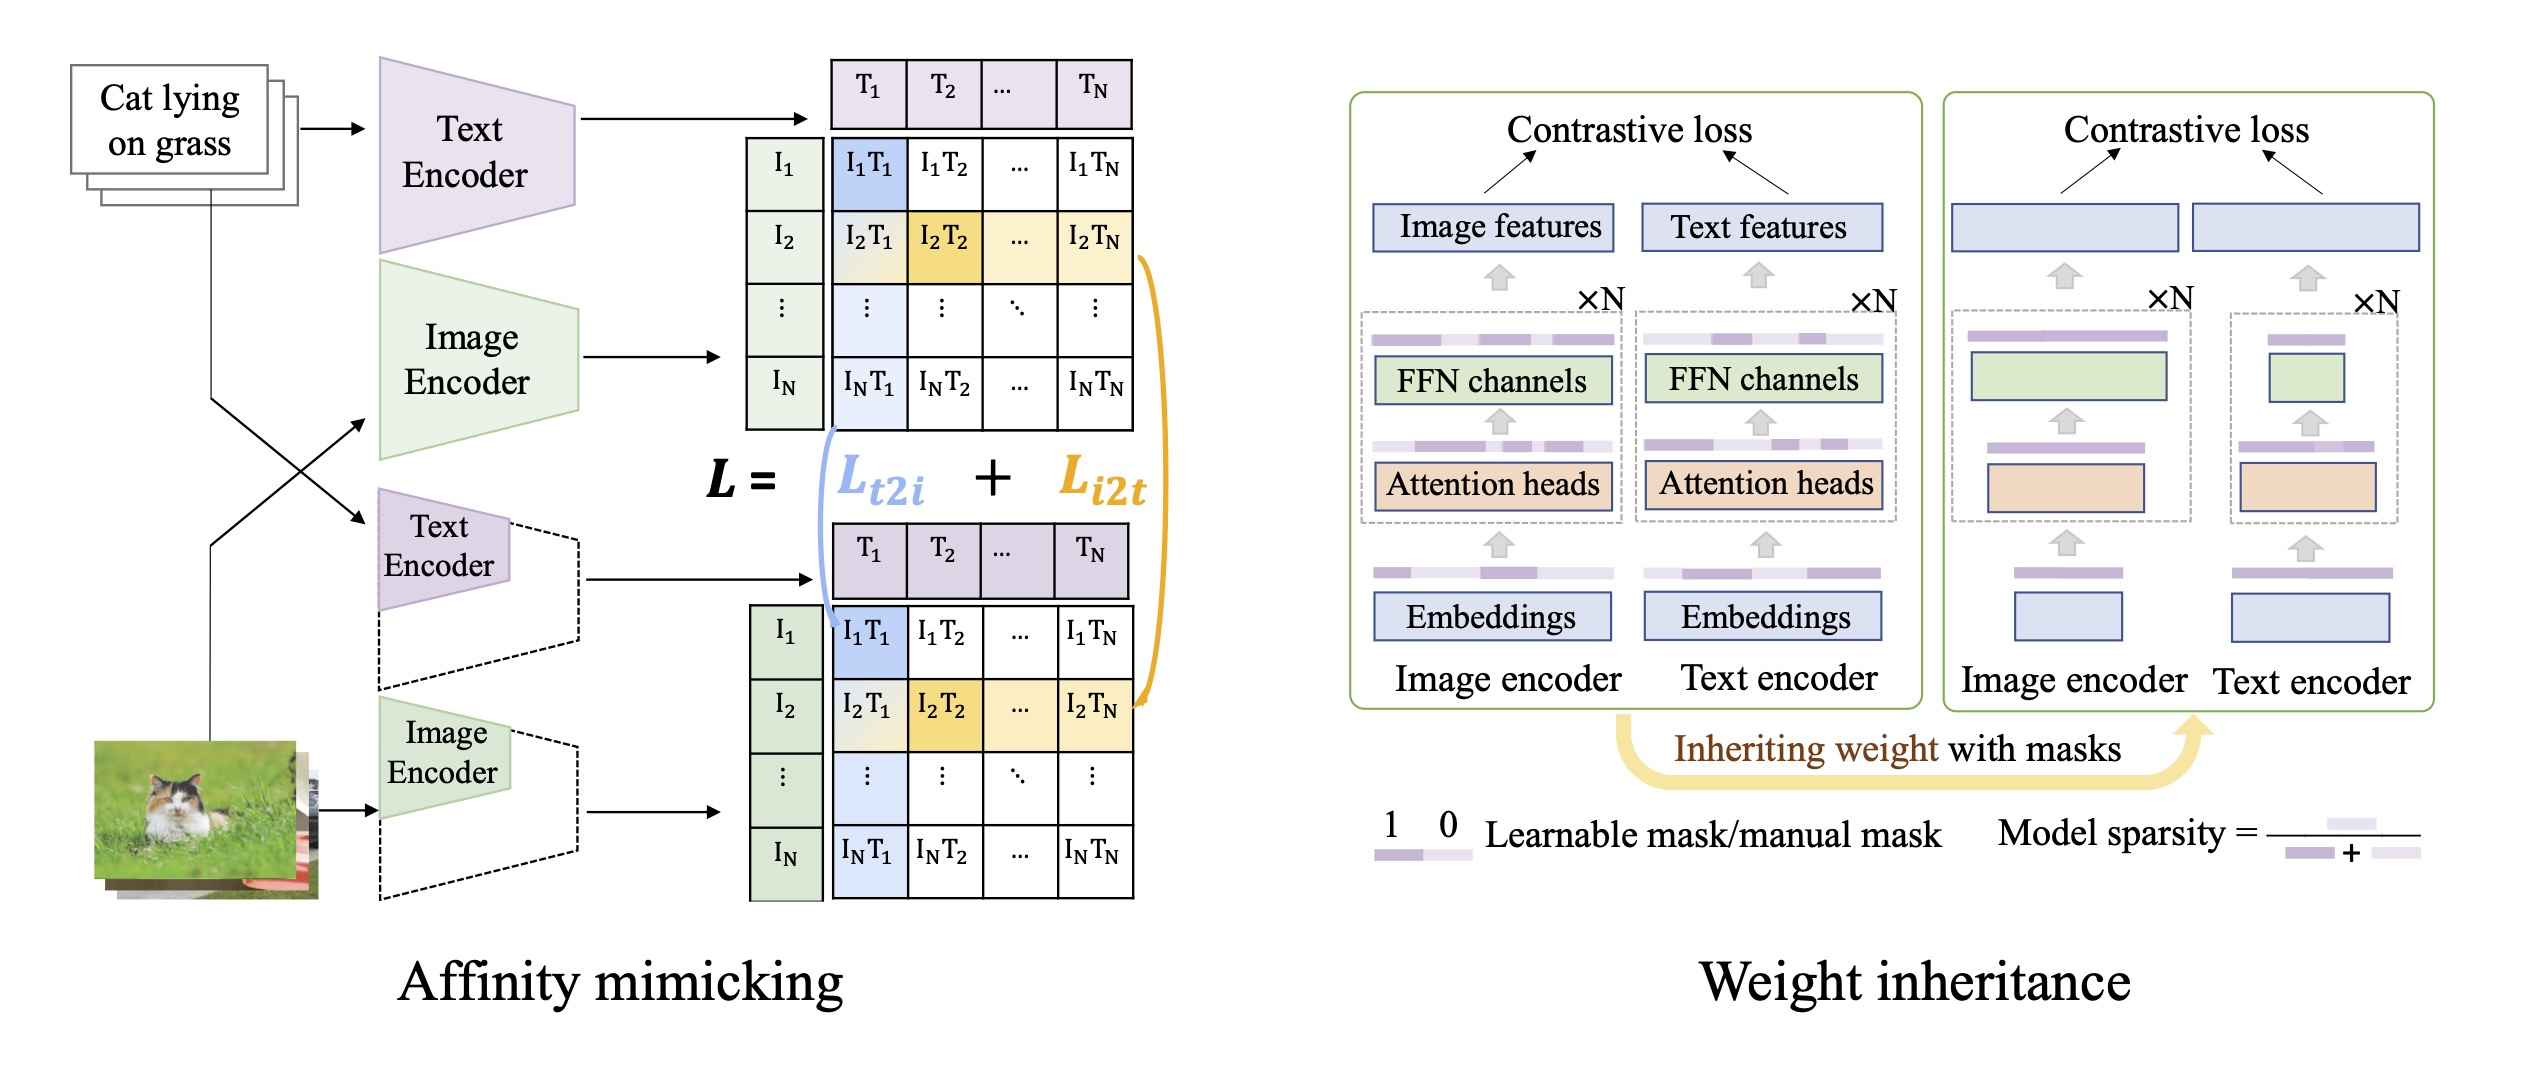
\includegraphics[width=\textwidth]{Images/crossmodalnetworks/TinyCLIP.jpg}
            \caption{Optimization which are used in TinyCLIP\cite{tinyclip}}
            \label{fig:crossmodalnetworks:tinyclip}
        \end{figure}

        TinyCLIP\cite{tinyclip} is a cross-modal distillation method for large-scale pre-trained speech-image models.
TinyClip can be used on limited systems due to its miniaturisation.
        It also speeds up training with minimal loss of model accuracy.
        It uses 3 concepts to reduce the size of the network.

        \subsubsection{Affinity mimicking}
        Affinity mimicking is a special form of knowledge distillation, also called model distillation.
        In knowledge distillation, a larger teacher network is trained first.
        After training the teacher network, a smaller student network is trained to predict the output of the teacher network.
        This works because the output of the teacher network has more information than the original label.
        Affinity Mimicking uses two new metrics in training: language-to-image loss and image-to-language loss (\(L_{t2i}\) and \(L_{i2t}\) in \cref{fig:crossmodalnetworks:tinyclip}).

        \subsubsection{Weight inhertiance}
        Weight inheritance is a technique that inherits important weights from well-trained teacher models to smaller student models.
        In the paper, the authors propose 2 methods:

        \subsubsection{Manual weight inhertiance}
        Based on the observations of the authors.
        Text encoders have most redundancy in depth (layer-wise), image encoders in width (channel-wise).
        They select \(k\) layers and channels of a branch, which will act as initialisation weights.
        To select the most important weights, some prior knowledge is required

        \subsubsection{Automatic weight inhertiance}
        The authors introduce a learnable mask to identify the importance of weight.

        \subsubsection{Multi-stage progressiv distillaiton}
        Pruning the model in several steps.
        For each stage, the authors use a modest degree of compression (e.g. 25\%). Each stage includes weight inheritance and affinity mimicking.

        % Due to the fact that TinyCLIP is already available and is much smaller in comparison to the origibal it will be further used in this work.

\section{Enhance the algorithm}

    To improve the accuracy of a pre-trained network, it can be fine-tuned to a specific task.
    Fine-tuning is a broad term.
    It ranges from the simple addition of a learnable linear layer at the end of the network to feature destillation.
    The concept of fine-tuning is derived from transfer learning\cite{transferlearning}.
    In transfer learning, the final layers of a neural network are removed and the network is retrained with new, independent layers.
    This saves time and resources.
    For example, with CLIP, a linear layer can be added to improve classification performance \cite{finetuneclip}.
    All of the fine-tuning approaches found use the output of the networks for further processing.
    Another way to increase the accuracy is to use better fitting text prompts.

    % \subsection{Probing}
    % % https://openaccess.thecvf.com/content/CVPR2024/papers/Huang_LP_A_Surprisingly_Strong_Linear_Probe_for_Few-Shot_CLIP_CVPR_2024_paper.pdf
    % \subsection{Feature destillation}
    % % https://arxiv.org/abs/2110.04544
    % \subsection{Prompt engeneering}

\section{Conclusion multi-modal networks}
    Based on the results of our own testing, ALIGN is not considered as a solution for this work.
    Instead, the focus of this work is on CLIP and TinyCLIP.
    These models can be fine-tuned to further improve their performance.
    In addition, the performance of the models can be improved by using better text prompts.
    \chapter{Hailo}

Based on recommendations from the advisors and the avilability, the Raspberry AI kit was used for this work.
It constist of a Hailo-8L entry level hardware accelerator.
Hailo provides a software called the \Acrfull{dfc} to convert a Tensorflow or ONNX model to a \Acrfull{hef}.
The Hailo hardware accelerator can execute \acrshort{hef} files on the Raspberry Pi.
Further information can be found in the \textit{Hailo Dataflow Compiler User Guide}.
    \chapter{Market analysis
\label{chapter:marketanalysis}}

Part of this work involves conducting a market analysis of hardware accelerators with M.2 interfaces. 
The results are summarized in the attached tables, highlighting the most relevant and significant details of these products.

\section{Summary of Current Offerings}
Many hardware accelerators available today have limitations that affect their suitability.
Some products, such as the Coral M.2 accelerator, are outdated and lack the processing power.
Other products, such as the SAKURA-II M.2 and Metis M.2 cards, are still only available for pre-order, limiting their accessibility for immediate use.

From the current assessment, the Hailo products appear to be the most promising options for this project.
They offer an efficient balance of performance and power consumption, outperforming Coral's offerings in terms of TOPS (tera operations per second) while maintaining a lower power footprint.
This efficiency is critical for embedded and power-sensitive applications, making Hailo a strong candidate for further exploration and integration.

\section{Future Considerations}
Looking ahead, hardware accelerators that can handle floating-point models (FP32 or BF16) offer exciting potential.
While integer (INT8) operations are optimized for many AI applications due to their efficiency, the theoretical advantages of FP32 precision for certain tasks warrant further investigation.
However, the practical benefits of this precision shift remain to be demonstrated in many real-world use cases.


\section{Custom Design Opportunities}
An alternative to relying on off-the-shelf solutions is to design and manufacture custom PCBs with M.2 slots.
This approach enables more tailored integration and reduces dependency on proprietary vendor software.  
Many companies offer hardware accelerator chips that can be incorporated into custom designs, providing the flexibility to optimize the hardware for specific application requirements.


\section{Software Ecosystem}
In addition to the hardware, the software ecosystem that accompanies these accelerators is a critical consideration.
The entire solution, including both hardware and software, must be ready for seamless deployment.
Many companies offer end-to-end software stacks to simplify integration and accelerate development. For example:

\begin{itemize}
    \item \textbf{Hailo} offers tools such as the Dataflow Compiler \acrshort{dfc} and GStreamer/Python APIs.
    \item \textbf{Axelera} supports its products with the Voyager.SDK.
\end{itemize}

Despite these offerings, assessing the usability of software stacks during initial evaluations remains a challenge.
Most documentation and sample applications focus primarily on computer vision tasks, potentially limiting their applicability to broader use cases.
Further practical testing is required to fully understand the ease of integration and the adaptability of these tools.


\section{Detailed Tables}
The tables below summarize the economic and technical key figures of the hardware accelerators reviewed, providing a comparative overview of their capabilities and specifications.
In \cref{tab:market:keyfigures}, we see that some accelerators support BF16.
BF16 stands for Brain Floating Point with 16 bits. This format uses less space than FP32 while still being a floating-point representation.
A blank cell in the tables indicates that no information was found.

\begin{table}[!ht]
    \centering
    \begin{tabular}{|l|l|l|l|l|}
    \hline
        Product Name & Manufacturer & Price (\$) & Availability & \makecell{M.2 Slot\\Type (Key)} \\ \hline
        Hailo-8L Entry-Level M.2 Module & Hailo & 80 & Available & M, B+M, A+E \\ \hline
        Hailo-8 M.2 AI Acceleration Module & Hailo & 220 & Available & M, B+M, A+E \\ \hline
        Hailo-10H M.2 Key M & Hailo & ~ & On request & M \\ \hline
        Metis M.2 Card & Axelera & 150 & Preorder & M \\ \hline
        SAKURA-II M.2 & Edge Cortix & 249-299 & Preorder & M \\ \hline
        M.2 Accelerator & Coral & 25 & Available & B+M, A+E \\ \hline
        M.2 Accelerator Dual Edge TPU & Coral & 40 & Available & E \\ \hline
        ME1076 M.2 Accelerator Card & Mythic & ~ & On request & A+E \\ \hline
        MM1076 M.2 Accelerator Card & Mythic & ~ & On request & M \\ \hline
        MLSoC Dual M.2 Production Board & Sima.ai & ~ & On request & Dual M.2 \\ \hline
        MemryX MX3 & MemryX & ~ & On request & N.A.(Chip) \\ \hline
        Orca 1.1 M.2 & DeGirum & 159 & Available & M \\ \hline
        byteENGINE IMX8MP Plus Quad & bytesatwork & 139 & Available & N.A.(Chip) \\ \hline
        Jetson Orin Nano 4GB & Nvidia & ~ & ~ & N.A.(Chip) \\ \hline
        Jetson Orin Nano 8GB & Nvidia & ~ & ~ & N.A.(Chip) \\ \hline
        Jetson Orin Nano Developer Kit & Nvidia & ~ & ~ & N.A.(Chip) \\ \hline
        EnCharge AI Analog IMC & EnChargeAI & ~ & ~ & ~ \\ \hline
    \end{tabular}
    \caption{Economical key figures of reviewed hardware accelerators.}
    \label{tab:market:ecotable}
\end{table}

\begin{table}[!ht]
    \centering
    \begin{tabular}{|l|l|l|l|}
    \hline
        Product Name & \makecell{Processing\\Power\\(TOPS INT8)} & \makecell{Processing\\Power\\(TFLOPS FP32)} & \makecell{Power\\Consumption} \\ \hline
        Hailo-8L Entry-Level M.2 Module & 13 & ~ & 1.5 W \\ \hline
        Hailo-8 M.2 AI Acceleration Module & 26 & ~ & 2.5 W \\ \hline
        Hailo-10H M.2 Key M & 40 & ~ & 3.5 W \\ \hline
        Metis M.2 Card & 214 & ~ & 4-8 W \\ \hline
        SAKURA-II M.2 & 60 & 30 (BF16) & 10 W \\ \hline
        M.2 Accelerator & 4 & ~ & 2 W \\ \hline
        M.2 Accelerator Dual Edge TPU & 8 & ~ & 4 W \\ \hline
        ME1076 M.2 Accelerator Card & 25 & ~ & 3.5 W \\ \hline
        MM1076 M.2 Accelerator Card & 25 & ~ & 3.5 W \\ \hline
        MLSoC Dual M.2 Production Board & 50 & ~ & 15 W \\ \hline
        MemryX MX3 & ~ & 5 (BF16) & ~ \\ \hline
        Orca 1.1 M.2 & ~ & ~ & 4.5 W \\ \hline
        byteENGINE IMX8MP Plus Quad & 2.3 & ~ & 33 W \\ \hline
        Jetson Orin Nano 4GB & 20 & ~ & 7-10 W \\ \hline
        Jetson Orin Nano 8GB & 40 & ~ & 7-15 W \\ \hline
        Jetson Orin Nano Developer Kit & 40 & ~ & 7-15 W \\ \hline
        EnCharge AI Analog IMC & 150  & ~ & ~ \\ \hline
    \end{tabular}
    \caption{Key technical figures of reviewed hardware accelerators.}
    \label{tab:market:keyfigures}
\end{table}

    % ==================================================
    % Quellen
    %%\input{text/Theorie.tex}
    \newpage
    \input{common/selbstständigkeits.tex}
    \newpage
    % ==================================================
    % Verzeichnisse
    \pagenumbering{alph}
    \printbibliography
    \listoffigures
    \listoftables
    \newpage
    
\end{document}

